\documentclass[10pt]{article}
\usepackage[margin=1in]{geometry}
\usepackage{graphicx,booktabs,amsmath,amssymb,xcolor,caption,enumitem,multirow,placeins}
\usepackage[hidelinks,colorlinks=true,linkcolor={blue!55!black},citecolor={blue!55!black},urlcolor={blue!55!black}]{hyperref}
\captionsetup{font=small,labelfont=bf,width=.94\textwidth}
\setlist{itemsep=2pt,topsep=3pt}
\newcommand{\seq}{\textsc{seq}}
\newcommand{\pl}{\textsc{par}}
\newcommand{\hr}[1]{\texttt{#1}}
\graphicspath{{figs/}}

\title{\textbf{BeliefLens: Belief Dynamics in LLM Forecasting Harnesses}\\[2pt]
\Large Technical Report}
\author{BeliefLens Project\\\small Deep Digital Intelligence \; · \; \url{https://github.com/DDI-droid/belieflens}}
\date{September 10, 2026 \; · \; v1.1}

\begin{document}
\maketitle

\begin{abstract}
LLM forecasters are \emph{judgmental} forecasters: behind every stated probability is something
that behaves like a belief, and behind every revision an update rule. BeliefLens measures both.
Four \emph{harness shapes} (\hr{react}, \hr{futuresim}, \hr{analytica}, \hr{bayesian})---prompt-defined
re-implementations of each source system's reasoning structure, with shape-specific state-carry
code, executed by one shared single-agent tool loop on a 339{,}801-article date-gated news
corpus---forecast real
January--March 2026 events under two protocols: \textbf{sequential} (five dates in order, own
history carried; $k{=}5$ rollouts) and \textbf{parallel} (fresh one-shot per date; $k_2{=}5$
rollouts), so every belief is a distribution. From each trajectory we \emph{recover the reasoning
as a literal-free program}: named variables extracted from the reasoning are the only values a
synthesized program may use, and blind sample/temporal holdouts decide whether the recovered
method is real. Findings: reasoning-structure stability and evidence tracking
\emph{anticorrelate}; \hr{bayesian}'s reasoning is a genuine fixed formula (its early-days
program predicts held-out late days at MAE $\approx0.003$) and its sequential trajectory is
unbiased against its own fresh-eyes belief; \hr{futuresim}'s rigidity decomposes into history
anchoring (update gain $-0.14$, the only negative), procedure-level conservatism, and---under
direct evidence---full rule compliance; \hr{react}'s updates flow through channels no recoverable
program contains. All 1{,}432 logged searches replay with zero articles past the date gate, and
an independent adversarial review is incorporated with every correction documented
(\S\ref{sec:audit}).
\end{abstract}

\section{Introduction}
Benchmarks such as FutureSim~\cite{futuresim} score LLM forecasting agents on outcomes, and observe
behaviours---anchoring to initial forecasts, ``self-conditioning'' on past rationales---that are
claims about \emph{belief dynamics}. But a score cannot say where a pathology lives: in what the
agent \emph{believes}, in how it \emph{updates}, or in how it \emph{gathers evidence}. This report
develops instrumentation that separates those layers, and applies it to four widely used reasoning
shapes.

The central device is \textbf{program recovery} (\S\ref{sec:e2}). If a harness's day-to-day
reasoning is a stable method applied to changing inputs, then a single program---with \emph{no
numeric literals anywhere}, only named quantities extracted from the reasoning itself---should
reproduce every forecast the harness made, with only the variable bindings changing between days.
The program is then the \emph{reasoning structure}; the bindings are the \emph{belief state}; and
the split is forced by construction, because the literal ban leaves a number nowhere to hide.
Once such a program exists, belief dynamics become measurable: the belief is a trajectory in the
program's own coordinates, and the program is an executable referee for counterfactual probes
(\S\ref{sec:probe}).

\paragraph{Contributions.}
\begin{itemize}
\item \textbf{Infrastructure.} A replayable forecasting environment on the real FutureSim corpus
(339{,}801 articles, 2025-12-01--2026-03-31) with an SQL-enforced date gate verified by
\emph{replaying all 1{,}432 logged searches} (zero breaches); four harness shapes on one substrate
so that reasoning structure is the only manipulated variable; dual elicitation protocols
(sequential $k{=}5$, parallel $k_2{=}5$) yielding belief \emph{distributions}, not points.
\item \textbf{Method.} A literal-free program space with a mechanical anti-gaming validator (no
literals, no boolean constants, no constant-only arithmetic, no value-spelling names such as
\texttt{two=2}, no dead code, no $x/x$), an answer-copy filter over raw/odds/percent/complement
transforms, and blind sample/temporal holdouts as the deciding gate; a standing audit that
re-verifies all of it against collected data.
\item \textbf{Findings.} A stability--plasticity inversion across harnesses; recovery of a true
fixed update formula for \hr{bayesian}; a three-way decomposition of \hr{futuresim}'s rigidity
(acquisition, procedure, and history---but \emph{not} rule violation); quantified conservatism
(update gains $0.22$--$0.47$, all $<\!1$) with \hr{futuresim} negative; and the incompressibility
of free-form ReAct reasoning.
\end{itemize}

\section{Background}
\textbf{Analytica}~\cite{analytica} decomposes a query into a tree of soft propositions, grounds
leaves with tools, and composes upward with a linear rule, arguing bias falls at the leaves and
variance in the composition. \textbf{FutureSim}~\cite{futuresim} replays dated news past model
cutoffs and documents anchoring and self-conditioning in frontier agents.
\textbf{Agent-BRACE}~\cite{agentbrace} represents an agent's belief as atomic claims with ordinal
certainty and shows such beliefs grow calibrated as evidence accrues. Our harnesses instantiate
these three shapes (plus a plain ReAct~\cite{react} floor); our measurements ask the question none
of the three answers: whether the externalized structure \emph{is} the working belief, and what
moves it.

\section{Experimental Infrastructure}\label{sec:infra}
\subsection{Corpus and date gate}
Articles are the FutureSim corpus (HF \texttt{shash42/forecast-news}; CCNews-derived,
deduplicated, dated): 120 day-partitions, 2025-12-01--2026-03-31, indexed to SQLite FTS5 (BM25),
339{,}801 rows. At simulation date $D$ the one search tool returns only articles with
$\text{date} \le D$; the constraint is in the SQL, not the prompt. \emph{Verification:} the audit
re-executes every search any harness ever logged (483 in the main runs, 949 in the scale-up) with
its turn's date; zero returned articles postdate the gate. We do not use FutureSim's 48\,GB
prebuilt hybrid index; retrieval (BM25) is weaker than the paper's but byte-identical across
harnesses, so it is a constant of the experiment, not a confound in it.

\subsection{Harnesses}
\textbf{What these are, precisely.} All four run on \emph{one} shared code path: a
single-agent tool loop (at most five \texttt{search\_news} rounds, then a forced answer, output
contract \texttt{FORECAST:\,$p$}). What differs per harness is (i) the system prompt imposing the
reasoning structure and (ii) a small amount of shape-specific code---for \hr{futuresim} and
\hr{bayesian}, programmatic extraction of the memory/belief block and its re-injection the next
day. They are therefore \emph{prompt-level re-implementations of each source system's reasoning
shape}, not the source systems themselves: real Analytica builds its proposition tree and computes
its linear composition \emph{in orchestration code} with parallel per-leaf grounder agents; the
real FutureSim harness maintains task state as an executable dataframe with structured memory
tools; the BLF system adds multi-trial aggregation and calibration. Our \hr{react} coincides with
its source (ReAct \emph{is} a prompt pattern over a tool loop); the others approximate.
This is a deliberate control---installing the papers' repositories would compare repositories,
whereas holding the substrate fixed makes reasoning shape the only manipulated variable---but it
bounds the claims: every cross-harness result in this report is a statement about reasoning
shapes at fixed capacity, \textbf{not} an evaluation of the source systems.
Table~\ref{tab:harness} summarises.

\begin{table}[tbp]\centering\small
\begin{tabular}{@{}llll@{}}
\toprule
harness & structure imposed & carries across days & lineage \\
\midrule
\hr{react} & free think/search loop & forecast history$^{\ast}$ & ReAct~\cite{react} \\
\hr{futuresim} & 6 ordered guidelines; base rate first; & history + memory block & FutureSim
baseline \\
 & forced $\le$200-word memory update & & harness~\cite{futuresim} \\
\hr{analytica} & decompose 3--5 sub-propositions $\to$ ground & forecast history$^{\ast}$ &
Analytica~\cite{analytica} \\
 & each by search $\to$ synthesize with weights & & \\
\hr{bayesian} & prior $\to$ evidence $\to$ per-item likelihood & history + belief block &
sequential Bayesian \\
 & ratio $\to$ posterior; forced belief block & & updating~\cite{blf} \\
\bottomrule
\end{tabular}
\caption{The four reasoning shapes. $^{\ast}$All four see their own prior forecasts in the
sequential protocol (the anchoring pressure, applied uniformly); \hr{react} is therefore a
\emph{history-anchored} floor, not a memoryless one.}
\label{tab:harness}
\end{table}

\subsection{Model choice and contamination}
Harnesses run on \texttt{gpt-5-mini} (released 2025-08-07): the questions resolve January--March
2026, so any later model would \emph{recall} rather than forecast, and a model that knows the
outcome does not move its belief---destroying the dynamics measurement. The extractor
(\texttt{gpt-5.2}) post-dates the events; it writes variables and programs but makes no forecasts,
and its one leakage channel (tilting extracted values toward the known outcome) is audited via the
preserved pre-reconciliation variable tables: across 320 tables, exactly one systematically
answer-tracking variable was found (\texttt{posterior\_odds}, odds-form, 10/10 instances), and no
recovered program references it.

\subsection{Questions}
The paired control: \emph{Will the USA / will Canada win the Milano-Cortina men's hockey gold?}
(one evidence stream; resolves YES/NO). Both teams won their semifinals on 02-20---the last
simulated date---and the final resolved 02-22, \emph{outside} the window; a correct forecaster
therefore raises \emph{both} beliefs toward $\sim$0.5, and the proper metrics are coherence
metrics---both beliefs rising across the semifinal (\emph{semi-rise}) and
$P_\text{USA}{+}P_\text{CAN}\!\to\!1$---not directional separation. (Our
original design scored directional separation; the adversarial review, \S\ref{sec:audit}, showed it
would have punished correct forecasting, and it was replaced before any conclusion was drawn.)
A scale-up set of four further questions from the OpenForesight dataset (FutureSim's question
source) supports the recovery statistics of \S\ref{sec:e2}; all four resolve YES, a bias we
disclose and therefore exclude from directional claims.

\section{The Literal-Free Program Space}\label{sec:dsl}
A recovered program is one Python function \texttt{forecast()} over an injected namespace, with:
\textbf{(R1)} no numeric, string, or \emph{boolean} literals anywhere; \textbf{(R2)} no
user-defined functions, imports, attributes, subscripts, comprehensions, or containers (recursion
and \texttt{while} permitted; execution carries a 200k-step budget so non-termination is a failed
fit); \textbf{(R3)} calls only to eleven whitelisted operations (\texttt{clamp},
\texttt{logistic}, \texttt{noisy\_or}, \texttt{odds}, \texttt{prob}, \texttt{min/max/abs/round/
exp/log/sqrt}) and nine named constants; \textbf{(R4)} \emph{no value may hide in a name}:
\texttt{two=2}, \texttt{half=0.5}, \texttt{const\_0\_62} are rejected in variable tables, schemas,
and program locals alike; \textbf{(R5)} no constant-only arithmetic
(\texttt{TENTH*(TWO+TWO+TWO)}\,$=$\,a smuggled $0.6$), no self-ops ($x{-}x$, $x/x$), no dead code
(\texttt{ZERO*(\dots)}, identity ops, unused locals). An eleven-exploit battery (including all
constructions found by the adversarial review) must reject under the validator and does; a
legitimate program passes. Because in-sample fit with visible targets cannot by itself distinguish
structure from memorisation, \textbf{the deciding gate is out-of-sample}: programs are
re-synthesized on a subset whose complement's targets the synthesizer never sees.

\section{Experiment 1: Replay}\label{sec:e1}
\subsection{Protocols}
\textbf{Sequential (\seq)}: five dates in order (01-14, 01-28, 02-08, 02-15, 02-20); each day the
harness sees its own previous forecasts (and its carry block) and may search the gated corpus;
$k{=}5$ independent rollouts of the whole trajectory. \textbf{Parallel (\pl)}: for each date, a
fresh single-shot run given all information up to that date and \emph{no} history; $k_2{=}5$
rollouts per date. Day~1 of a sequential rollout is, by construction, a parallel draw---a built-in
sanity check (12/16 day-1 sequential values fall inside the day-1 parallel spread at $\pm 0.05$).
All 560 collected forecasts parse under the strict parser (200 sequential + 200 parallel on the
pair, plus 160 scale-up; no fallback; percent and comma handled; out-of-range triggers a retry),
and every stored forecast re-parses identically from its own turn text.
Figure~\ref{fig:flow} shows the resulting trajectories.

\begin{figure}[tbp]\centering
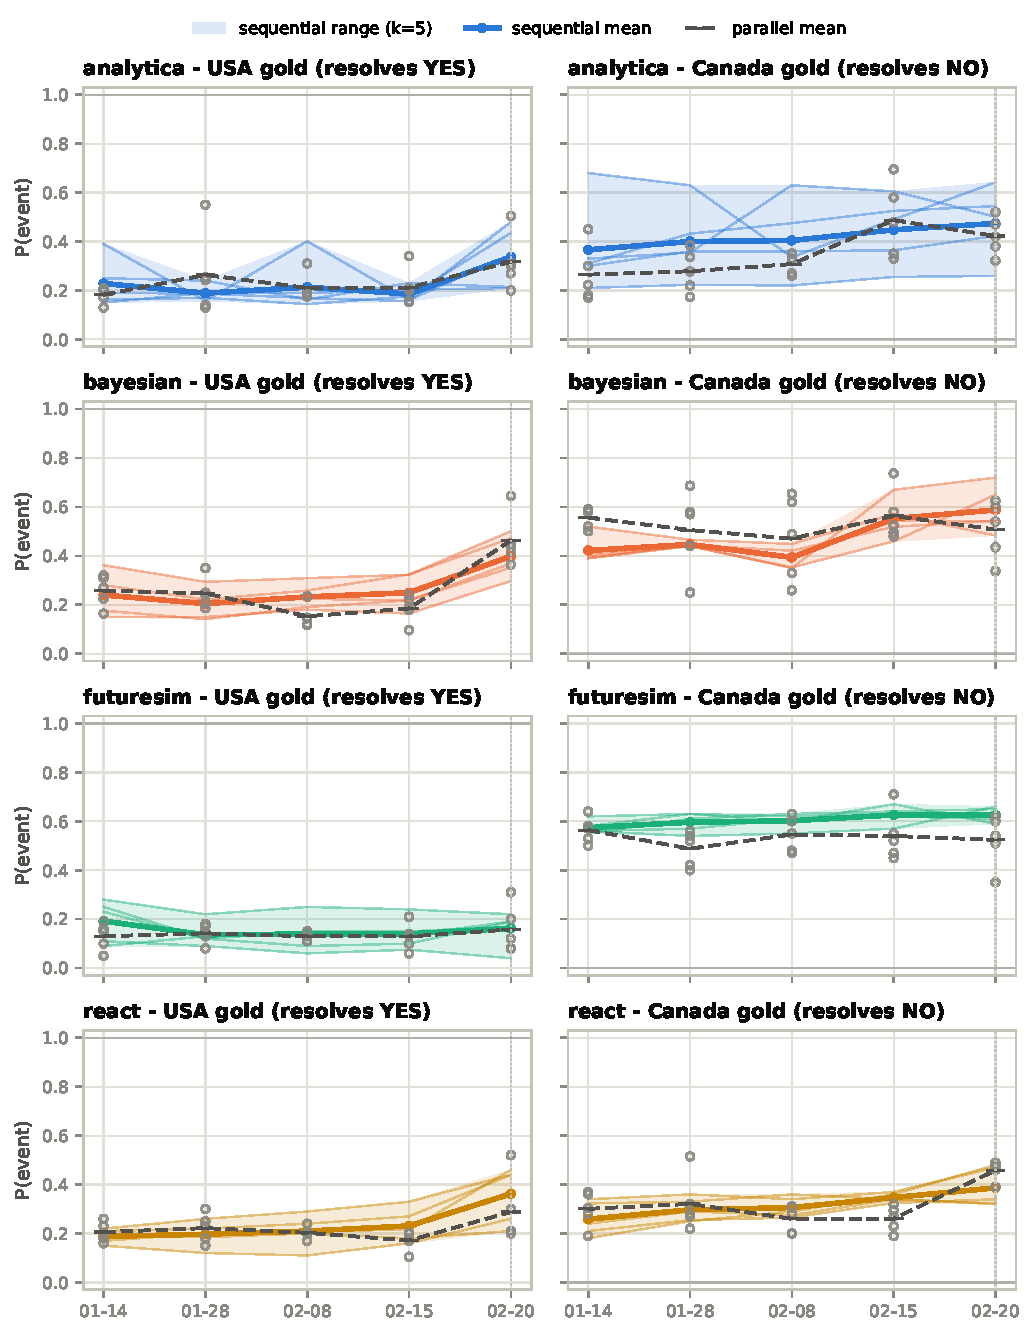
\includegraphics[width=.98\textwidth]{fig_flow.pdf}
\caption{\textbf{Belief flow, all four harnesses on the paired questions.} Shaded band and bold
line: range and mean of the five \seq{} rollouts (history carried). Open dots and dashed line: the
five \pl{} one-shot draws per date and their mean (fresh eyes on the same evidence). Dotted
vertical: semifinal date. \hr{futuresim}--Canada's band rides above its fresh-eyes mean (anchoring)
and \hr{futuresim}--USA barely responds even in \pl{} (procedure-level conservatism);
\hr{bayesian} hugs its fresh-eyes mean in both panels.}
\label{fig:flow}
\end{figure}

\subsection{Metrics}
For dates $t\ge2$: \textbf{anchor gap} $=\seq_t-\overline{\pl}_t$ (signed; what carrying history
does relative to evidence alone); \textbf{lag advantage} $=|\seq_t-\overline{\pl}_t| -
|\seq_t-\overline{\pl}_{t-1}|$ (positive $\Rightarrow$ the sequence tracks \emph{yesterday's}
evidence-conditioned belief better than today's); \textbf{update gain} $=$ OLS slope of
$\Delta\seq_t$ on $\Delta\overline{\pl}_t$ (1 $=$ moves with the evidence; $<\!1$ conservatism);
\textbf{placement} $=$ percentile of each \seq{} forecast within that date's \pl{} draws
(50 $=$ unbiased); \textbf{stabilisation} $=\mathrm{sd}(\seq)/\mathrm{sd}(\pl)$ per date;
\textbf{coherence} $=P_\text{USA}{+}P_\text{CAN}$ (\textbf{sum@last} is its value on 02-20);
\textbf{total movement} $|\Delta|_\text{tot}$, the summed absolute day-to-day change of a rollout;
and \textbf{Brier}~\cite{brier}. Placement is a probability-integral-transform (PIT) statistic,
and PIT$_{\mathrm{med}}$ its median. Figures~\ref{fig:gain}--\ref{fig:coh} render these;
Table~\ref{tab:e1} summarises. Throughout this report,
Brier is the plain quadratic score $\frac1n\sum_i(p_i-y_i)^2$ with $y_i\in\{0,1\}$ the resolved
outcome, pooled over the pair---\emph{not} a skill score (no baseline subtraction, no
$1{-}\mathrm{MSE}$ orientation, no difficulty adjustment); 0 is perfect, 0.25 is the constant-0.5
forecaster.

\begin{table}[tbp]\centering\small
\begin{tabular}{@{}lrrrrrrrr@{}}
\toprule
& \multicolumn{3}{c}{replay (\seq, $k{=}5$)} & \multicolumn{5}{c}{\seq{} vs \pl}\\
\cmidrule(lr){2-4}\cmidrule(l){5-9}
harness & $|\Delta|_\text{tot}$ & semi-rise & sum@last & gap & $|$gap$|$ & gain & lag adv. &
PIT$_{\mathrm{med}}$\\
\midrule
\hr{analytica} & 0.331 & 0.60 & 0.81 & $+0.019$ & 0.098 & 0.22 & $-0.009$ & 60 \\
\hr{bayesian}  & 0.283 & \textbf{0.80} & \textbf{0.99} & $\mathbf{-0.004}$ & 0.072 &
\textbf{0.47} & $-0.028$ & 40 \\
\hr{futuresim} & \textbf{0.134} & \textbf{0.00} & 0.79 & $\mathbf{+0.046}$ & 0.067 &
$\mathbf{-0.14}$ & $\mathbf{+0.003}$ & \textbf{80} \\
\hr{react}     & 0.182 & 0.60 & 0.75 & $+0.019$ & 0.066 & 0.27 & $-0.011$ & 60 \\
\bottomrule
\end{tabular}
\caption{\textbf{E1 headline metrics} ($k{=}5$ both conditions; pooled over the pair). Semi-rise:
fraction of rollouts in which \emph{both} paired beliefs rose across the semifinal date (the
correct direction). \hr{bayesian} is the best coherent tracker and is unbiased against its own
fresh-eyes belief; \hr{futuresim} never raised both after the semifinals, carries the largest
anchor gap, is the only harness with positive lag advantage, and its update gain is
\emph{negative}---together consistent with tracking yesterday's evidence-conditioned belief
rather than today's. Bold marks, per column, the value most indicative of anchoring or of its
absence.}
\label{tab:e1}
\end{table}

\begin{figure}[tbp]\centering
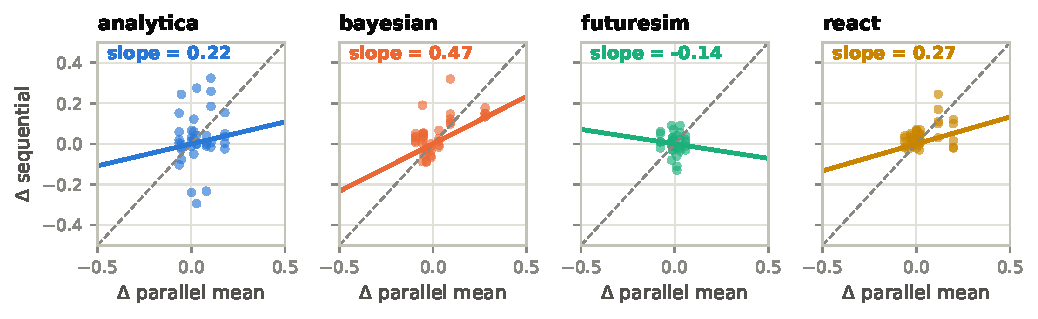
\includegraphics[width=.98\textwidth]{fig_gain.pdf}
\caption{\textbf{Update gain.} Each dot is one date-step: $x$, movement of the fresh-eyes mean;
$y$, movement of a sequential rollout. Dashed: $y{=}x$. All fitted slopes are below 1
(conservatism); \hr{futuresim}'s is negative.}
\label{fig:gain}
\end{figure}

\begin{figure}[tbp]\centering
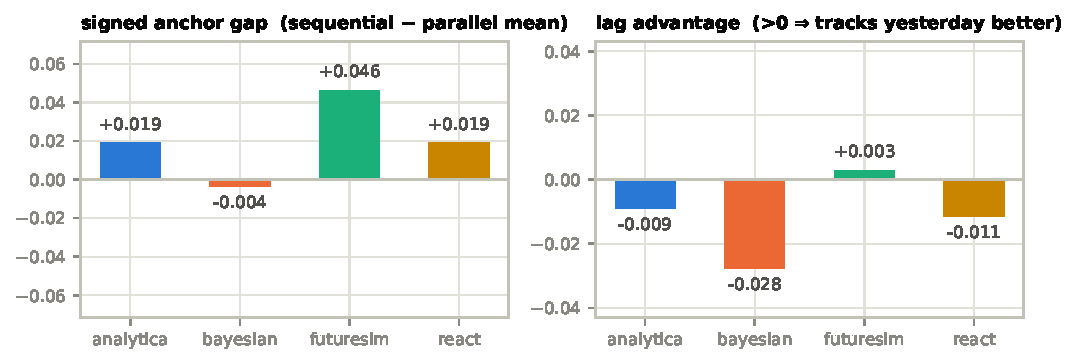
\includegraphics[width=.9\textwidth]{fig_anchor.pdf}
\caption{\textbf{Anchoring summary.} Left: signed anchor gap. Right: lag advantage; only
\hr{futuresim} is positive.}
\label{fig:anchor}
\end{figure}

\begin{figure}[tbp]\centering
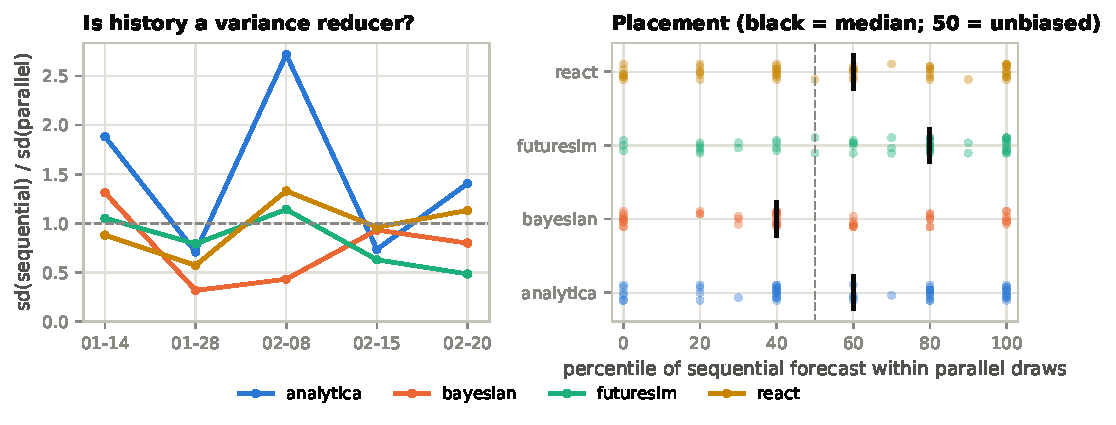
\includegraphics[width=.98\textwidth]{fig_stab_pit.pdf}
\caption{\textbf{Left:} stabilisation ratio $\mathrm{sd}(\seq)/\mathrm{sd}(\pl)$. History acts as
a variance reducer where the ratio sits below 1 (\hr{futuresim}, \hr{react}); \hr{analytica}'s
ratio above 1 on several dates is path dependence---rollouts diverge because their own early draws
differed. \textbf{Right:} placement of every sequential forecast within its date's fresh-eyes
distribution; \hr{futuresim}'s median sits at the 80th percentile (anchored high), \hr{bayesian}'s
at the 40th.}
\label{fig:stab}
\end{figure}

\begin{figure}[tbp]\centering
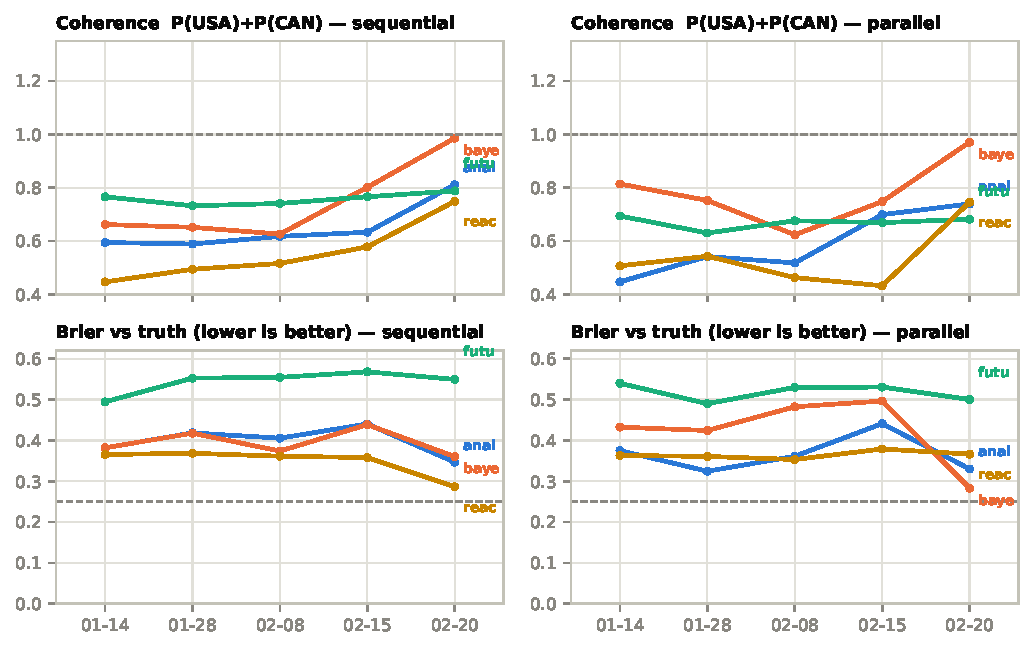
\includegraphics[width=.98\textwidth]{fig_coh_brier.pdf}
\caption{\textbf{Coherence and accuracy by condition.} Top: $P_\text{USA}{+}P_\text{CAN}$ should
approach 1 by the semifinal (dashed). Bottom: plain Brier against the resolved outcomes (lower is
better), pooled over the pair.}
\label{fig:coh}
\end{figure}

\subsection{Search effort}
Mean searches per turn (\seq{} / \pl): \hr{analytica} 7.3/6.8, \hr{futuresim} 6.6/6.2,
\hr{react} 5.3/5.0, \hr{bayesian} 5.0/5.5. Memory does not substitute for retrieval at this
scale; \hr{analytica}'s per-sub-proposition grounding makes it the heaviest searcher in both
conditions (a truncation covariate logged per turn as \texttt{forced\_stop}).

\FloatBarrier
\section{Experiment 2: Program Recovery}\label{sec:e2}
\subsection{Pipeline}
For every forecast turn: \textbf{step 1}, the extractor reads that day's searches and reasoning
and emits \texttt{name = value} declarations for every quantity the reasoning used---never the
output, in any parameterisation (raw, odds, percent, complement all dropped within $\pm0.005$;
yesterday's forecast exempted as the legitimate anchor input); names must describe world
quantities, never values. \textbf{Step 2} reconciles the per-day tables into one canonical schema
(missing instance keys retried once, then excluded loudly---never zero-filled; pre-reconciliation
tables preserved as the audit trail). \textbf{Step 3} synthesizes \emph{one} program per
harness--question against all ($\le$10) instances, repaired against validator violations and worst
residuals for at most four attempts; then re-synthesizes \emph{blind} on (a) sample~0 only and (b)
the first three dates only, evaluated untouched on the held-out complement.
Figure~\ref{fig:recovery} and Table~\ref{tab:e2} give the results.

\begin{figure}[tbp]\centering
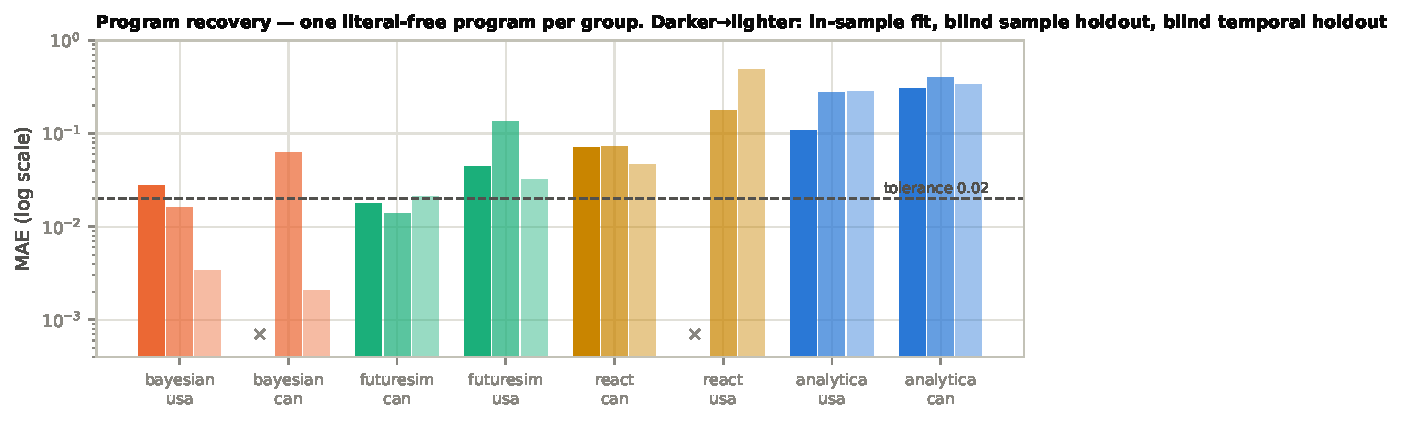
\includegraphics[width=.98\textwidth]{fig_recovery.pdf}
\caption{\textbf{Recovery quality per group} (log MAE; $\times$ marks ``no valid program'').
\hr{bayesian}'s blind temporal holdouts reach MAE 0.002--0.003: a genuinely fixed update formula.
\hr{analytica} fits poorly under every regime---its structure changes day to day. \hr{react}--USA
admits no program at all.}
\label{fig:recovery}
\end{figure}

\begin{table}[tbp]\centering\small
\begin{tabular}{@{}lrrrp{4.6cm}@{}}
\toprule
group & in-sample & sample-holdout & temporal (early$\to$late) & reading \\
\midrule
\hr{bayesian}/USA & 0.027 & \textbf{0.016} & 0.0005$\,\to\,$\textbf{0.003} & fixed log-odds formula \\
\hr{bayesian}/CAN & --- & 0.063 & 0.0003$\,\to\,$\textbf{0.002} & same; full-fit failed to execute \\
\hr{futuresim}/CAN & \textbf{0.018} & \textbf{0.014} & 0.015$\,\to\,$0.021 & stable; both halves
recover the \emph{identical} program \\
\hr{futuresim}/USA & 0.045 & 0.135 & 0.051$\,\to\,$0.032 & stable-ish \\
\hr{react}/CAN & 0.070 & 0.073 & 0.044$\,\to\,$0.046 & weak method \\
\hr{react}/USA & none & 0.178 & 0.252$\,\to\,$0.487 & incompressible \\
\hr{analytica}/USA & 0.108 & 0.274 & 0.073$\,\to\,$0.285 & \multirow{2}{*}{\parbox{4.4cm}{structure changes daily (in-context shape; \S\ref{sec:limits}, item 8)}} \\
\hr{analytica}/CAN & 0.301 & 0.396 & 0.520$\,\to\,$0.335 & \\
\bottomrule
\end{tabular}
\caption{\textbf{Program-recovery MAE.} Holdout columns are blind (targets hidden from the
synthesizer); bold marks MAE at or below the 0.02 tolerance. No group passes the strict gate
\emph{on the full in-sample fit} (MAE $\le 0.02$ $\wedge$ $\ge$80\% of instances within tolerance
$\wedge$ 0 failures), so in-sample fits are reported as descriptive---but two blind holdouts
individually meet every threshold (\hr{futuresim}/CAN sample-holdout: 0.014 at 80\% in-tolerance,
0 failures; \hr{bayesian} temporal: 0.002--0.003 at 100\%), and the blind columns are the honest
evidence throughout. Scale-up (four further questions, 16 groups, hardened rules): 10 clean, 5 marked
recovery-uninformative (near-constant targets make both copy-detection and recovery ill-posed),
1 no-program.}
\label{tab:e2}
\end{table}

\begin{figure}[tbp]\centering
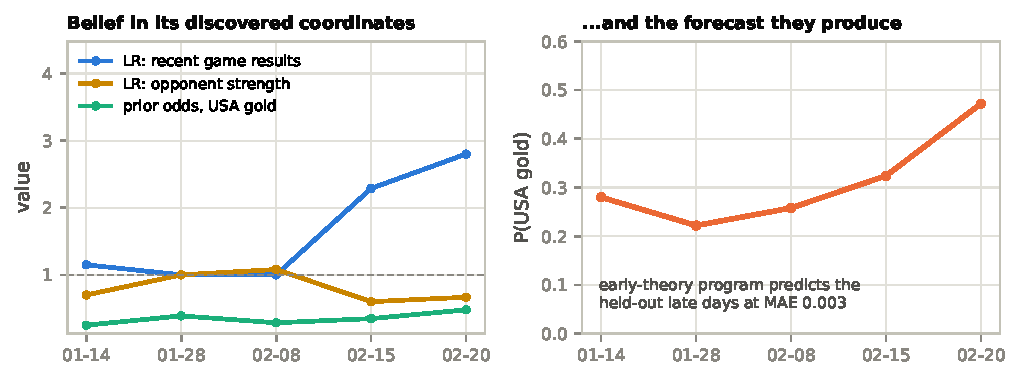
\includegraphics[width=.98\textwidth]{fig_exemplar.pdf}
\caption{\textbf{The belief in its discovered coordinates} (\hr{bayesian}/USA, rollout s0). Left:
three recovered variables across the window---the recent-results likelihood ratio climbs
$1.1\!\to\!2.9$ as the USA advances while the prior odds ratchet behind it. Right: the forecast
those coordinates produce. The recovered programs are log-odds additive updating with a
shrink-to-prior term (full-fit version listed in Appendix~\ref{app:prog}); re-synthesized blind
on the first three dates alone, the temporal variant---same family, different expression---predicts
the last two days at the MAE shown.}
\label{fig:exemplar}
\end{figure}

\subsection{Residual drift and theory change}
Fitting one program across all dates makes \emph{failure} informative: \hr{analytica}/CAN's mean
$|$residual$|$ grows by $+0.34$ from first to last date (USA: $+0.05$)---its method decays---while
\hr{futuresim}'s is flat or improving (CAN $-0.007$, USA $-0.07$). Figure~\ref{fig:exemplar}
shows the recovered belief coordinates for the cleanest case. Function-space distance between the full-fit and
sample-0-only programs (Monte-Carlo over the observed binding box):
\hr{futuresim}/CAN \textbf{0.000} (identical theory from either half of the data),
\hr{bayesian}/USA 0.044, \hr{react}/CAN 0.174, \hr{analytica}/CAN 0.391.

\FloatBarrier
\section{The Rigidity Probe}\label{sec:probe}
Each probed harness was continued from its real end-of-run state to a probe day (02-21) with
search disabled (stated as an outage) and exactly one injected, role-based news item---``Canada's
starting goaltender ruled out of the final'' / the USA mirror / an irrelevant placebo. Its own
recovered program supplies the referee twice over: a \emph{single-coordinate} implied change
(perturb only the targeted variable), and a \emph{multi-coordinate} rule-implied forecast
(re-extract the probe day's full bindings from the harness's own reasoning and execute the
program). Placebo movements were $\le0.02$; \textbf{all sixteen directional probes (4 groups $\times$ 2
rollouts $\times$ 2 directions) moved the correct direction}. Figure~\ref{fig:probe} and
Table~\ref{tab:verdict} summarise.

\begin{figure}[tbp]\centering
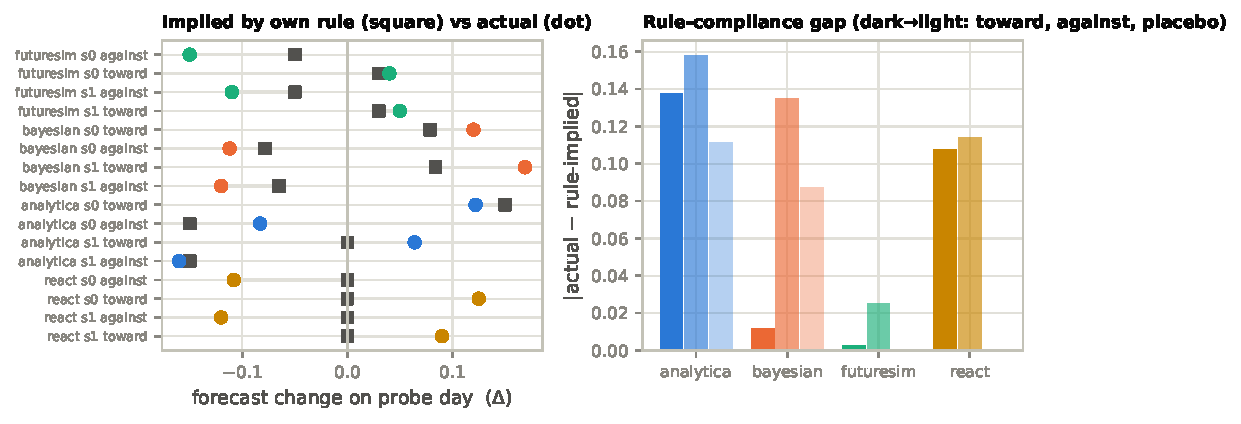
\includegraphics[width=.98\textwidth]{fig_probe.pdf}
\caption{\textbf{Left:} single-coordinate implied change (square) vs actual change (dot) for every
directional probe. \textbf{Right:} the multi-coordinate rule-compliance gap
$|p_{\text{actual}}-p_{\text{rule}}|$ by condition. \hr{futuresim}'s gaps are $\le0.04$: handed
the evidence, it computes with its recovered structure almost exactly. \hr{react}'s program
implies zero response in every cell while the live harness moved $\pm0.09$--$0.13$: its updates
use machinery its recoverable structure does not contain.}
\label{fig:probe}
\end{figure}

\begin{table}[tbp]\centering\small
\begin{tabular}{@{}lcccl@{}}
\toprule
harness & method stable? & tracks evidence? & honours own rule? & diagnosis \\
\midrule
\hr{futuresim} & yes & poorly in replay & \textbf{yes} (gap $\le$0.04) & rigidity lives in
\emph{acquisition}, \\
& & & & \; not revision \\
\hr{bayesian} & yes & good & asymmetric & compliant on good news; over-drops \\
& & & & \; on bad news vs own rule ($\approx\!-0.135$) \\
\hr{react} & no & yes & n/a (rule has no channel) & updates outside recoverable structure \\
\hr{analytica} & no & good & no verdict possible & rewrites its method daily \\
\bottomrule
\end{tabular}
\caption{\textbf{Per-harness verdicts}, combining \S\ref{sec:e1}--\S\ref{sec:probe}. The one-line
finding: structural stability and evidence-tracking anticorrelate, and the probe \emph{localises}
each harness's rigidity or plasticity.}
\label{tab:verdict}
\end{table}

\FloatBarrier
\section{Adversarial Review and Standing Audit}\label{sec:audit}
Mid-experiment, an independent reviewer was pointed at the entire codebase with instructions to
break it. It returned 2 fatal, 7 serious, and 6 moderate findings; every fixable one was patched
and re-verified before results were trusted. The fatals: (F1) the planned ``separation'' metric
would have punished correct forecasting given the actual event path (\S\ref{sec:infra}); (F2) the
no-literal rule was semantically bypassable (constant-construction, boolean arithmetic,
if-chain lookup tables coached by the repair loop)---closed by the rules of \S\ref{sec:dsl} plus
the blind holdouts. Serious findings included a thread-unsafe SQLite connection that corrupted 32\%
of an early run (that run is quarantined and unused), a forecast parser that could fabricate
certainty from ``85\%'' (fixed; the strict parser reproduces all collected forecasts exactly), and
silent zero-filling in schema reconciliation (replaced by loud exclusion plus a preserved audit
trail). The standing audit (\texttt{scripts/audit\_exp1.py}) re-verifies on demand: 11/11 exploits
rejected; all 560 collected forecasts parse under the strict parser (the 240 audited retroactively
re-parse identically); 1{,}432 searches replayed with zero gate breaches; every stored program re-executes to its reported MAE; one systematic answer-copy in 320
variable tables, referenced by no program.

\FloatBarrier
\section{Limitations}\label{sec:limits}
(1) One question pair carries all directional claims; the scale-up set is all-YES by construction
and supports only recovery statistics. (2) $k{=}5$ per cell bounds distributional claims; PIT
placement has 5-draw granularity. (3) Draws are ordinary decoding variation (current reasoning
endpoints reject temperature control). (4) Stated beliefs only: all measurements are consistency
properties of verbalized probabilities under intervention, not claims about internal
representations. (5) Retrieval is BM25, weaker than FutureSim's hybrid index---held constant
across harnesses, but absolute accuracy is a lower bound. (6) The extractor knows the outcomes;
the audit bounds but does not eliminate this channel. (7) Program recovery inherits the
expressiveness of the program space; ``incompressible'' means no program \emph{in this space}
within four repair attempts. (8) The harnesses are prompt-level shapes on a shared loop
(\S3.2), not the source systems: in particular, real Analytica enforces its tree and linear
composition \emph{in code}, so ``\hr{analytica}'s structure changes daily'' characterises a
model asked to follow that procedure in-context, and would be prevented by construction in the
original system; conversely, \hr{bayesian}'s recovered fixed formula is the more striking for
being maintained by the model with no code enforcement.

\section{Conclusion and Future Work}
Treating a forecasting agent's reasoning as a recoverable, literal-free program turns belief
dynamics from a metaphor into a measurement: beliefs become trajectories in discovered
coordinates, updates become testable against the agent's own rule, and rigidity decomposes into
acquisition, procedure, history, and revision components that this report measures separately for
four harness shapes. Next: paired NO-questions and longer date grids; per-search-call budgets; a
code-execution harness as the recovery upper bound; program recovery on the parallel condition
(does removing history delete the anchor variables from the schema?); and alignment of the
\hr{bayesian} harness with its source paper's exact protocol.

\begin{thebibliography}{9}\small
\bibitem{analytica} \emph{Analytica: Soft Propositional Reasoning for Robust and
Scalable LLM-Driven Analysis}. arXiv:2604.23072, 2026.
\bibitem{futuresim} \emph{FutureSim: Replaying World Events to Evaluate Adaptive Agents}.
arXiv:2605.15188, 2026.
\bibitem{agentbrace} \emph{Agent-BRACE: Decoupling Beliefs from Actions in Long-Horizon Tasks via
Verbalized State Uncertainty}. arXiv:2605.11436, 2026.
\bibitem{react} \emph{ReAct: Synergizing Reasoning and Acting in Language Models}.
ICLR, 2023.
\bibitem{blf} \emph{Agentic Forecasting using Sequential Bayesian Updating of Linguistic Beliefs}.
arXiv:2604.18576, 2026.
\bibitem{brier} \emph{Verification of forecasts expressed in terms of probability}.
Monthly Weather Review, 1950.
\end{thebibliography}

\appendix
\section{A Recovered Program}\label{app:prog}
The \hr{bayesian}/USA program (full-fit). The blind variants recover the same log-odds-additive family, though not this exact expression. Note the absence of
literals; every quantity is a step-1 variable or a named constant. The schema contained an
odds-form copy of the answer (\texttt{posterior\_odds\_usa\_gold}); the program does not reference
it.
\begin{quote}\small\begin{verbatim}
def forecast():
    p0 = prior_probability_usa_gold
    o0 = prior_odds_usa_gold
    ln_prior_odds = log(o0)
    ln_lr_total = log(lr_roster_strength_positive)
    ln_lr_total += log(lr_opponent_canada_strength)
    ln_lr_total += log(lr_injury_and_replacements)
    ln_lr_total += log(lr_recent_game_results)
    ln_lr_total += log(lr_nhl_participation_logistics)
    ln_lr_total += log(lr_venue_or_media_sentiment)
    ln_post_odds = ln_prior_odds + ln_lr_total
    p_bayes = logistic(ln_post_odds)
    logit_p0 = log(p0) - log(ONE - p0)
    gap = ln_post_odds - logit_p0
    tight = ONE / (ONE + abs(gap))
    w = (HALF + tight) * HALF
    return p0 + w * (p_bayes - p0)
\end{verbatim}\end{quote}

\section{Reproduction}
\texttt{git clone https://github.com/DDI-droid/belieflens \&\& python bootstrap.py} downloads the
corpus ($\sim$412\,MB), builds the index, and runs the verification battery; \texttt{scripts/}
contains every stage (\texttt{run\_exp1.py} for \seq/\pl/E2, \texttt{audit\_exp1.py},
\texttt{beliefdyn.py}, \texttt{run\_probe.py}, \texttt{probe\_rule\_check.py},
\texttt{make\_charts.py}). All collected data, configs, and logs ship in \texttt{results/}.
\end{document}
